% mainfile: ../praca_magisterska_orbifoldy.tex
\chapter{Counting orbifolds} \label{counting occurrences}
%In this chapter we would care not only whether the pointis or is not in the spectrum -- we will 
%give a closer look of how many orbifolds have particular \Eoc. \\
%Our ultimate goal is to give the answer to the questions such as: \\
%- For a given $x \in \sigma$, how many orbifolds have $x$ as their \Eoc?\\
%- Why? Is there some underlying geometrical reason for that?\\
%- Can we characterise points $x \in \sigma$ that has the most orbifolds corresponding to them? \\
%- Is there any reasonable normalisation to counter the effect that there are 'more' 
%points as we go 
%to lesser values. (What we mean by 'more' was sted in) \\
%The first equstion we can tackle is steaming from the chapter \ref{order structure} 
%and it is -- Do $\speD$ and $\speS$ coincide? It is easy to answer that $\speD \neq \speS$ 
%(and we will do that along some harder questions in the moment), but do they coincide 
%starting from a sufficiently distant point? Or maybe, for every denominator, do they coincide 
%from a sufficiently distatn point? (Yes.) \\
%\todo{przenieść (przekopiować?) część może do futher direction}
%write about cyclic order

The central question of this section is: "given a rational number, how many orbifolds 
have that \Eoc ?". 
%The warning for this chapter is, that this question will remain unansweared, 
%however, we can provide some glimpse into the partial answear. 

%To answear this, we should 
%first check, whether for any number, there are only fihis numer is always finite.
%Secondly:
In \ref{finiteness}, we will show that for any number, there are only finitely many 
orbifolds with that \Eoc. 
In \ref{infiniteness} we will show the local unboundness of $\spe$. 
In \ref{dividing the problem}, we will divide the problem into two parts 
that will be discussed in chapter 
\ref{Counting orbifolds -- arithmetical part} and chapter 
\ref{Counting orbifolds -- combinatorical part} and discuss these parts briefly. 
%we will separate the problem of finding the exact number into 
%more arithmetical 
%part and one more combinatorial. 

%There are two aspects of counting occurensec
%Even three.
%One, we can state some finitness conditions -- this is useful, to sort out what questions 
%are meaningfull
%Then there are study of expressions of he form:
%arithmetical expresions
%and the study of cmbinatorics.

\section{Finiteness}\label{finiteness}

In this section, we will prove, that for any $x \in \sigma$ there are only finitely many orbifolds 
with the \Eoc\ equal to $x$. We will give two proofs of this fact. 

%Here we will show that for any $x \in \sigma$:
%\begin{itemize}
%\item for every $n \in \mathbb{N}$ there are only finitely many orbifolds 
%with the \Eoc\ greater or equal to $x$ and all orbipoints of order at most $n$
%\item there are finitely many orbifolds with an \Eoc\ equal to $x$. 
%\end{itemize}

%\begin{lemma}\label{sum_of_reciprocals_lemma}
%The function $\rho:\mathbb{N}^m \to \mathbb{Q}$, defined as:
%\begin{equation}
%\rho(n_1, \cdots, n_m) \coloneqq \sum_{i = 0}^m \frac{1}{n_i},
%\end{equation} 
%is finite-to-1.
%\end{lemma}
%\subsubsection{Proof.}


%\begin{theorem}\label{second_finiteness_theorem}
%For any $x \in \sigma$ there are only finitely many orbifolds 
%with the \Eoc\ equal to $x$.
%\end{theorem}
%\subsubsection{Proof.}

%\begin{observation}

%\end{observation}

\begin{observation}\label{limit of number of orbipoints lemma}
Let us observe, that since:
\begin{itemize} 
\item $\Delta(^*2) = -\frac{1}{4}$,
\item $\Delta(2) = -\frac{1}{2}$,
\item every $M$ with boundary has $\chi(M) \leq 1$,
\item every $M$ without boundary has $\chi(M) \leq 2$,
\end{itemize}
we have, that there can be at most 
$n \coloneqq \max \{\lfloor 4(1-x) \rfloor, \lfloor 2(2-x) \rfloor\}$ 
orbipoints at any orbifold with an \Eoc\ $\geq x$. 
\end{observation}

%\begin{theorem}
%Let $x$ be an accumulation point of order $0$ 
%\end{theorem}

\begin{observation}\label{first_finiteness_theorem}
For any $x \in \sigma$ and $n \in \mathbb{N}$ there are only 
at most 
\begin{equation}
(n-1)^{\max \{\lfloor 4(1-x) \rfloor, \lfloor 2(2-x) \rfloor\}}
\end{equation} 
orbifolds 
with the \Eoc\ greater or equal to $x$ and all orbipoints of order at most $n$.
\end{observation}
\subsubsection{Proof.} 

For a given $x$, there are only finitely many manifolds 
with an Euler characteristic $y \geq x$. Only them can be 
base manifolds for an orbifold with an \Eoc\ $y'\geq x$, as adding orbipoints always 
decreases an \Eoc. 

It remains to prove then, that for any base manifold $M$, there are only finitely many orbifolds, 
with $M$ as a base manifold, that have 
 an \Eoc\ $y \geq x$, and all orbipoints of order at most $n$.

%We proceed now similarly to the proof of \ref{finiteness_lemma} -- 
From \ref{limit of number of orbipoints lemma} we have that 
on the orbifold with an \Eoc\ $y \in [x,2]$, there can be at most 
$\max \{\lfloor 4(1-x) \rfloor, \lfloor 2(2-x) \rfloor\}$ orbipoints. 
Thus, for a given manifold $M$ and a given $x$ and $n$, there can be at most 
$(n-1)^{\max \{\lfloor 4(1-x) \rfloor, \lfloor 2(2-x) \rfloor\}}$ orbifolds with an \Eoc\ 
$y \geq x$, 
all orbipoints of order at most $n$ and $M$ as a base manifold.$_\square$ 

\begin{observation}\label{simplification of the finiteness theorem}
To prove that for any $x \in \sigma$ there are only finitely many orbifolds 
with the \Eoc\ equal to $x$, it is sufficient, to prove that 
for any $x \in \sigma$, for any two dimensional manifold $M$, there are only 
finitely many $M$-orbifolds with only one corresponding type of orbipoints (dihedral in the case 
$M$ has a boundary or rotational in the case $M$ dos not have a boundary), 
with the \Eoc\ equal to $x$.
\end{observation}
\subsubsection{Proof.}
Let $x$ be a rational number. 
Let $\mathcal{O}$ be the set of all orbifolds with 
an \Eoc\ equal to $x$. 
Those orbifolds can have different base manifolds. However, the set of base manifolds of 
orbifolds from $\mathcal{O}$ is finite, as there are only finitely many 
two dimensional manifolds with an Euler characteristic greater or equal to $x$ and an 
orbifold always has 
an \Eoc\ less or equal to the Euler characteristic of its underlying manifold. 

%We will now provide an argument that shows that for any base manifold $M$, the number 
%of $M$ orbifolds with \Eoc\ equal to $x$ is finite. It will complete the proof of our theorem.\\
From this, it is sufficient to prove, that for any base manifold $M$, 
the number of $M$ orbifolds 
with \Eoc\ equal to $x$ is finite.

Let $M$ be a two dimensional manifold. 
%For the sake of contradiction, assume, that there exists an infinite set $\mathcal{O}_M$
%of $M$-orbifolds such that $\mathcal{O}_M \subseteq \mathcal{O}$ 
%($\ast$)
If $M$ has no boundary it can't have dihedral orbipoints and we have the the thesis for manifolds 
without boundary.

If $M$ has a boundary, $M$-orbifolds 
%in $\mathcal{O}_M$ 
can have both rotational and dihedral orbipoints. 
%For the simplicity of the following part of the proof we want now to reduce this case 
%to a case 
%where only one type of the orbipoints is present. 
Let us observe, that every rotational orbipoint can be replaced by two dihedral orbipoints 
of the same order without changing the \Eoc. Thus, if there would be infinitely many 
$M$-orbifolds having both rotational and dihedral orbipoints, there would be 
also infinitely many $M$-orbifolds having only dihedral orbipoints. 
Thus in this case it is sufficient to prove that there are finitely many $M$-orbifolds 
that have only dihedral orbipoints. $_\square$

%We will now perform the proof of above statement in the case of dihedral orbipoints.
%The proof for rotational orbipoints is completely analogous. 

%Let us call the subset of $\mathcal{O}_M$ 
%that consists only of orbifolds with only dihedral orbipoints by $\mathcal{O}_M^d$.

\begin{theorem}\label{second_finiteness_theorem}
For any $x \in \spe$ there are only finitely many orbifolds 
with the \Eoc\ equal to $x$.
\end{theorem}

%\subsubsection{Proof.}
%Let us take $x\in \spe$. 
%%Using \ref{simplification of the finiteness theorem} 
%%We will use observation \ref{simplification} and prove, that for any $M$
%By using observation \ref{simplification of the finiteness theorem} it is only needed to prove, 
%that for any $M$, there are only finitely many $M$-orbifolds with only dihedral orbipoints 
%with \Eoc\ equal to $x$. 

%Let $M$, be a two dimensional manifold.  

\subsubsection{Proof I.} 

Let us take $x\in \spe$. 
By using observation \ref{simplification of the finiteness theorem} it is only needed to prove, 
that for any $M$, there are only finitely many $M$-orbifolds with only one 
corresponding type of orbipoints 
(rotational in the case $M$ has no boundary, dihedral in the case $M$ has a boundary), 
with \Eoc\ equal to $x$. 

% Suppouse, that there exists an orbifold with an \Eoc\ qual to $x$. Then, 
%Let $x$ be a rational number. 
%Let $\mathcal{O}$ be the set of all orbifolds with 
%an \Eoc\ equal to $x$. 
%Those orbifolds can have different base manifolds. However, the set of base manifolds of 
%orbifolds from $\mathcal{O}$ is finite, as there are only finitely many 
%two dimensional manifolds with an Euler characteristic greater or equal to $x$ and an 
%orbifold always has 
%an \Eoc\ less or equal to the Euler characteristic of its underlying manifold. 

%%We will now provide an argument that shows that for any base manifold $M$, the number 
%%of $M$ orbifolds with \Eoc\ equal to $x$ is finite. It will complete the proof of our theorem.\\
%It remains to prove, that for any base manifold $M$, the number of $M$ orbifolds 
%with \Eoc\ equal to $x$ is finite: 

%Let $M$ be a two dimensional manifold. 

For the sake of contradiction, assume, that the set $\mathcal{O}_M$
of $M$-orbifolds that have only one type of orbipoints and have \Eoc\ equal to $x$ is infinite 
%($\ast$)
.

%If $M$ has some boundary, orbifolds in $\mathcal{O}_M$ 
%can have both rotational and dihedral orbipoints. 
%For the simplicity of the following part of the proof we want now to reduce this case 
%to a case 
%where only one type of the orbipoints is present. 

%Let us observe, that every rotational orbipoint can be replaced by two dihedral orbipoints 
%of the same order without changing the \Eoc. Thus, if there would be infinitely many 
%orbifolds in $\mathcal{O}_M$ having both rotational and dihedral orbipoints, there would be 
%also infinitely many orbifolds in $\mathcal{O}_M$ having only dihedral orbipoints. 
%Thus it is sufficient to prove that there are finitely many orbifolds in $\mathcal{O}_M$ 
%that have only one type of the orbipoints. 

%%We will now perform the proof of above statement in the case of dihedral orbipoints.
%%The proof for rotational orbipoints is completely analogous. 

%Let us call the subset of $\mathcal{O}_M$ 
%that consists only of orbifolds with only dihedral orbipoints by $\mathcal{O}_M^d$.

Let $\mathcal{O}_M = \{O_i\}_{i \in I}$. 
For each $i$, let $s_i = (o^0_i, \cdots, o^{l_i}_i)$ be the list of degrees of 
the orbipoints  
of $O_i$ ordered in a decreasing manner. 
%written with decreasing orders of 
%dihedral points. 
So for each $i$ we have, that $o^0_i$ is 
the order of the orbipoint with the highest order of all the dihedral orbipoints of 
$O_i$. 
By \ref{first_finiteness_theorem} we know that if the set $\{o^0_i\}_{i \in I}$ 
would be bounded 
by some $n \in \mathbb{N}$, by \ref{sameness} 
it would mean, that $\mathcal{O}_M^d$ would be finite. As 
from our assumption for the contradiction, we have that $\mathcal{O}_M$ is not finite, we know
that the set $\{o^0_i\}_{i \in I}$ is unbounded. 
Let $\{i_n\}_{n\in \mathbb{N}} \subseteq I$ be a sequence of indices such that
$\{o^0_{i_n}\}_{n\in \mathbb{N}}$ is strictly increasing. 

%Let $\{a_n\}$ be the sequence such that $a_n = \frac{m_n-1}{m_n} \end{cases}$ if point 
%corresponding 
%to $m_n$ is an rotational point and $a_n = \frac{m_n-1}{2m_n}$ if point corre 
Let $\{a_n\}$ be the sequence such that $a_n = \Delta(o^0_{i_n})$.
Let $\{b_n\}$ be the sequence such that $b_n = \Delta(o^1_{i_n},
\cdots, o^{l_{i_n}}_{i_n})$. 
So for every $n$ we know that $\cho{O_{i_n}} = \chi(M) + a_n + b_n$. 
\begin{figure}[H]
\centering
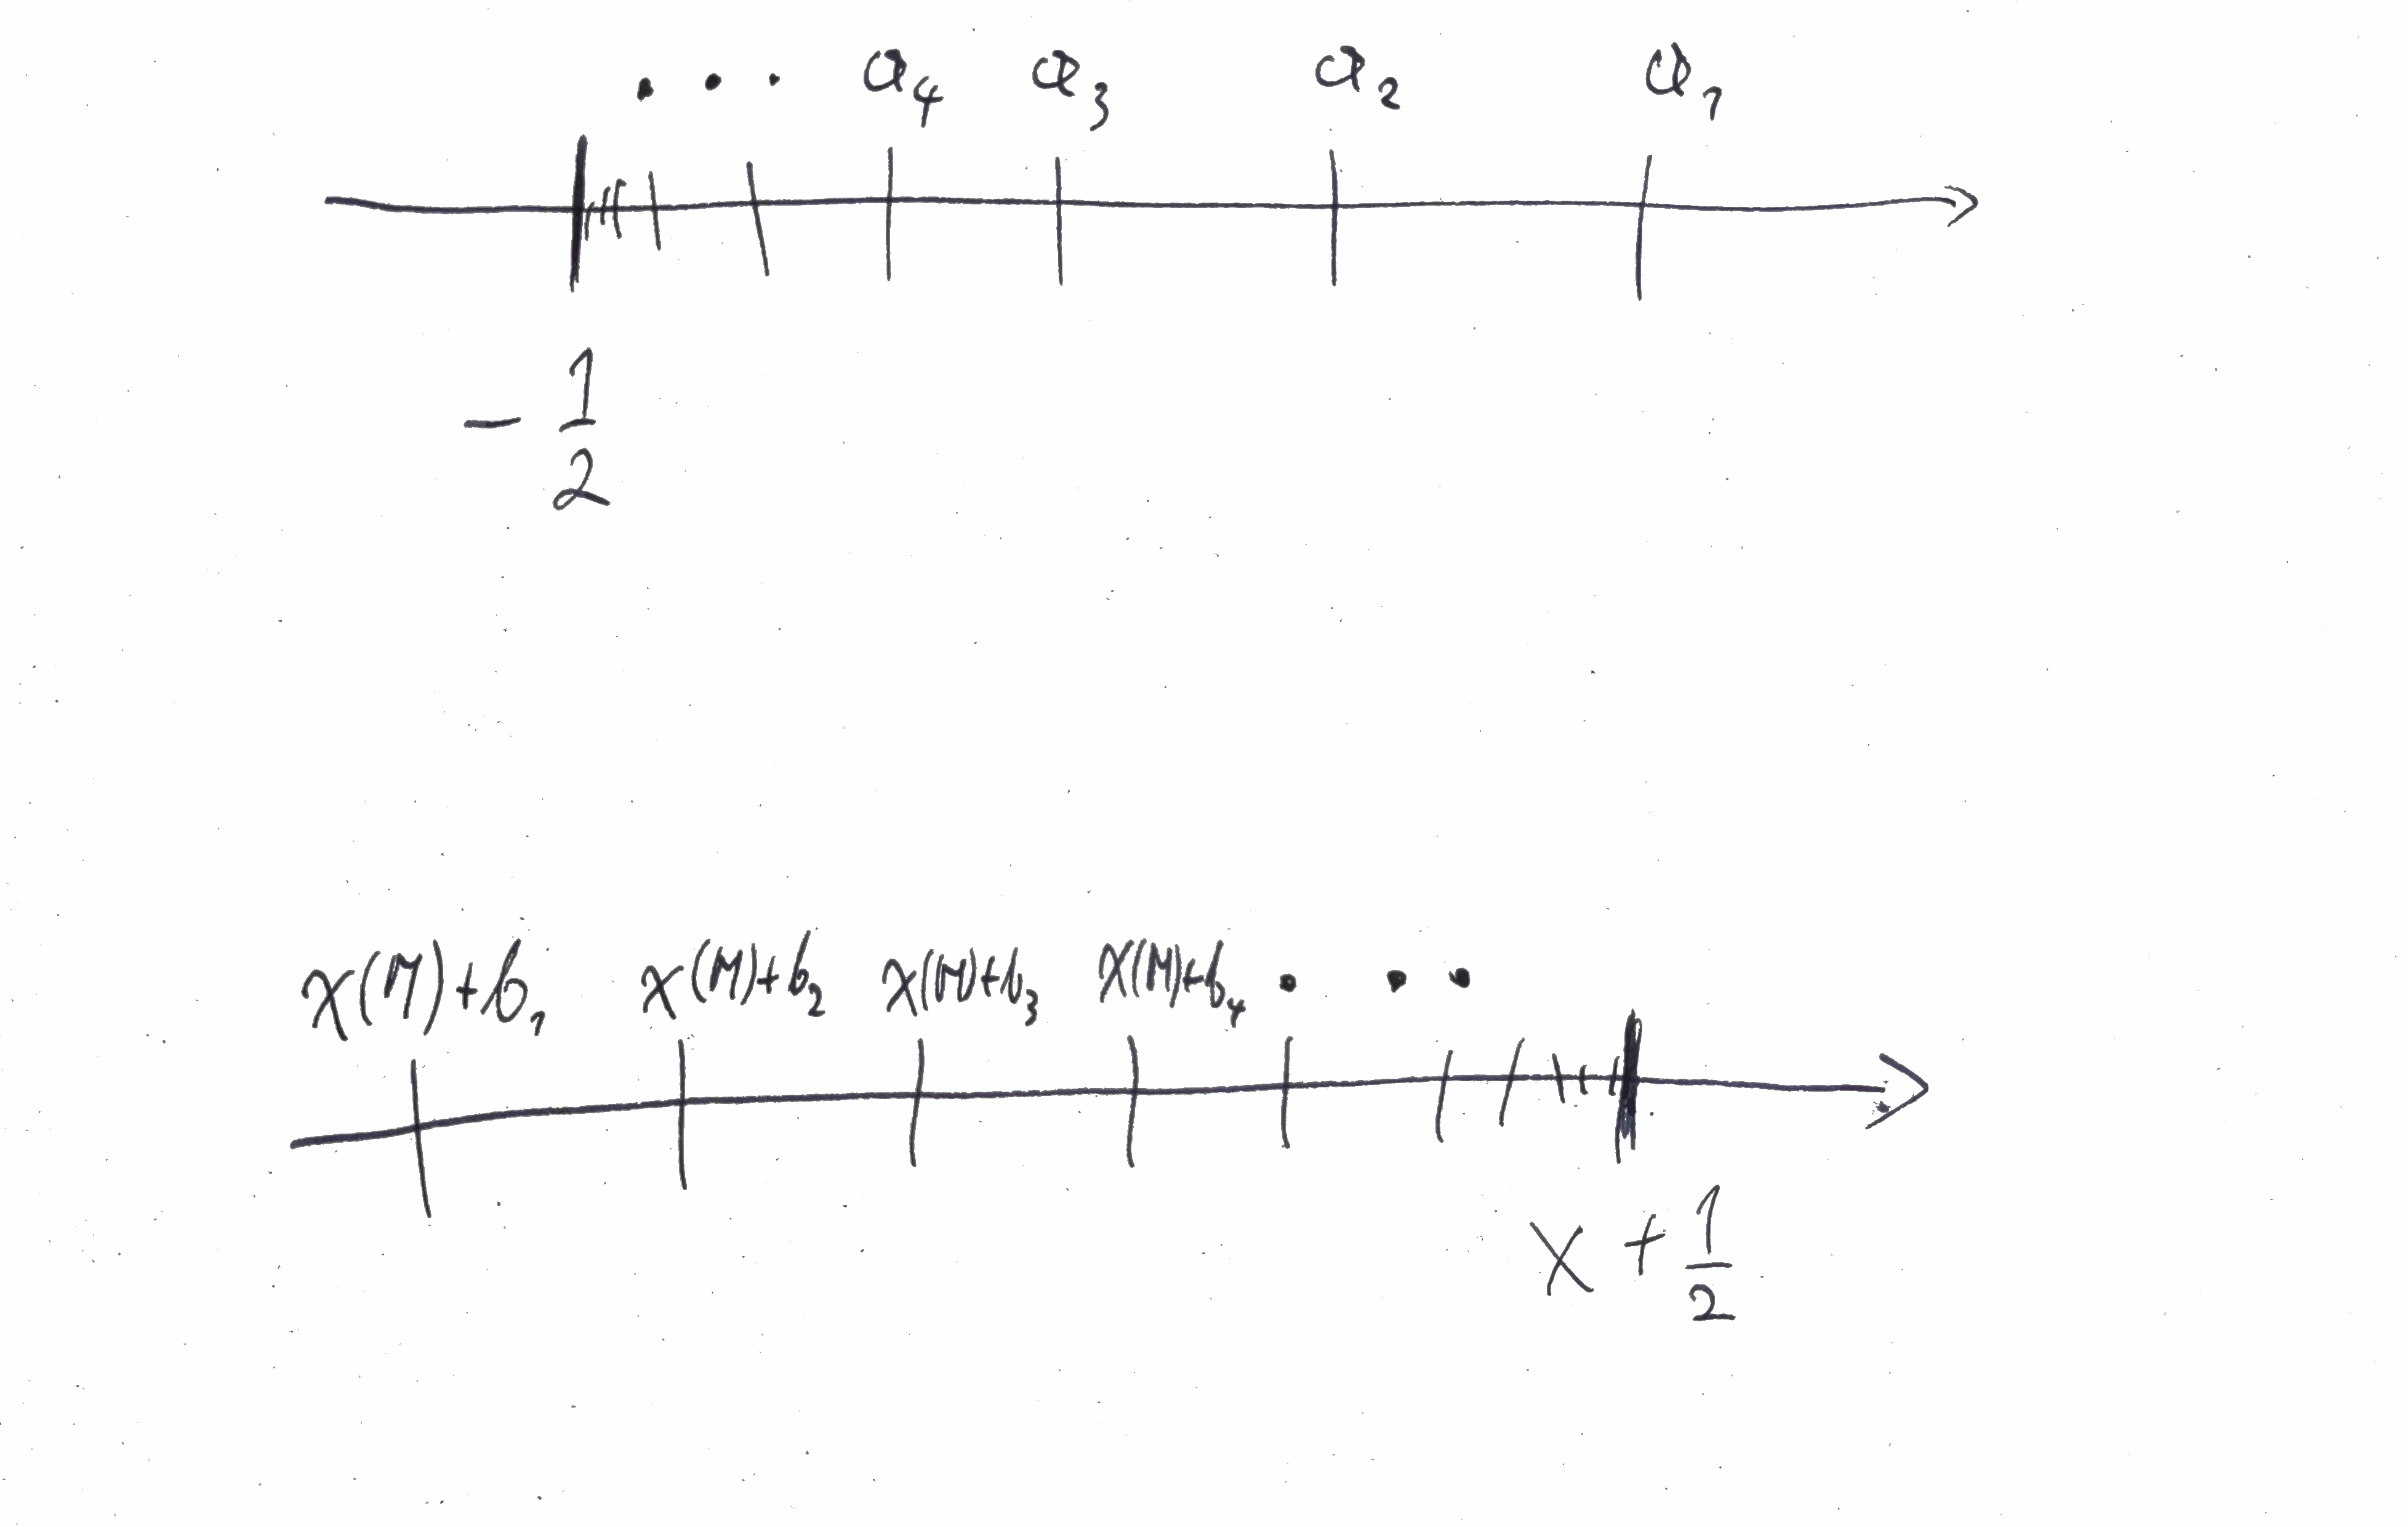
\includegraphics[width=\textwidth]{"../counting_orbifolds/anbn.jpg"}
\caption{Sequences $\{a_n\}$ and $\{\chi(M) + b_n\}$.}
\end{figure}
As $\{o^0_{i_n}\}$ 
is strictly 
increasing, we know 
that $a_n$ is strictly decreasing, so $b_n$ must be strictly 
increasing  
%(*), 
(we have that $\cho{O_{i_n}}$ is constant for all $n$, since all $O_{i_n}$ 
are from the family with \Eoc\ equal to $x$). 

But $\{b_n\} \subseteq \spebr{M} - \chi(M)$. 
From \ref{well_order} and \ref{all_spectra_are_isomorphic} we know that $\spebr{M}$ has no infinite 
strictly increasing sequences, so 
$\spebr{M} - \chi(M)$ has no infinite strongly increasing sequences. That gives us a 
contradiction. 
%*. 
%\Lightning 
$_\square$ 


%First we will show that for any $x \in \sigma$ there are always only finitely many orbifolds 
%with an \Eoc\ equal to $x$. \\ 
%Let us observe, that we only need to show this for $S^2$ orbifolds. It is like that, because, 
%as discussed in \ref{surgeries} every orbifold can be obtained be modyfying the sphere and 
%%the set of differences in \Eoc\ made by
%%all possible modifications that are not adding orbipoints is bounded. 
%there is only finitely many possible modifications that are not adding an orbipoint, each 
%changing \Eoc\ by non-zero value. \\ 

%\begin{theorem}
%For any $x \in \sigma$ there are always only finitely many orbifolds 
%with an \Eoc\ equal to $x$.
%\end{theorem}
%\textbf{Proof:} \\
%% Suppouse, that there exists an orbifold with an \Eoc\ qual to $x$. Then, 
%According to the note above, we only need to proof this for $S^2$ orbifolds. \\ 
%Let $x$ be a rational number. 
%For the sake of contradiction, assume, that there exists an infinite family of orbifolds 
%$\{\mathcal{O}\}_{i \in I}$ with an \Eoc\ of each qual to $x$. For each $i$, tet $m_i$ be the 
%order of the orbipoint with the highest order of $\mathcal{O}_i$. As for every $n \in \mathbb{N}$ 
%there are only finitely many $S^2$ orbifolds with all orbipoints of order less than $n$, we have 
%that the set $\{m_i\}_{i \in I}$ is unbounded. Let $\{m_n\}_{n\in \mathbb{N}}$ be some strictly 
%increasing sequence 
%of elements of $\{m_i\}_{i \in I}$ that diverges into infinity. \\
%Let $\{a_n\}$ be the sequence of differences in \Eoc\ caused by points corresponding 
%to $\{m_i\}$. 
%Let $\{b_n\}$ be the sequence of differences in \Eoc\ caused by other points on those orbifolds. 
%So for every $n$ we have $\cho{\mathcal{O}_n} = 2 + a_n + b_n$. As $\{m_n\}$ is strictly 
%increasing we have that $a_n$ is strictly decreasing, so $b_n$ must be strictly 
%increasing, because $\cho{\mathcal{O}_n}$ is constant for all $n$ (all $\{\mathcal{O}_n\}$ 
%are from the family with \Eoc\ equal to $x$). \\ 
%But $\{b_n\} \subseteq \speS - 2$, so it is well ordered as $\speS$ is well ordered. 
%From \ref{well_order} and \ref{times_two_fact} we know that $\speS$ has no infinite 
%strongly increasing sequences, so 
%$\speS - 2$ has no infinite strongly increasing sequences. That gives us a contradiction. 
%\Lightning $_\square$ 
 
\subsubsection{Proof II.}

Let us take $x\in \spe$. 
By using observation \ref{simplification of the finiteness theorem} it is only needed to prove, 
that for any $M$, there are only finitely many $M$-orbifolds with only one corresponding 
type of orbipoints 
(rotational in the case $M$ has no boundary, dihedral in the case $M$ has a boundary),
with \Eoc\ equal to $x$. 

%Similarly as in \ref{finiteness_lemma} and \ref{first_finiteness_theorem}, 
%we can deduce, that since:
%\begin{itemize} 
%\item $\Delta(^*2) = -\frac{1}{4}$,
%\item $\Delta(2) = -\frac{1}{2}$,
%\item every $M$ with boundary has $\chi(M) \leq 1$,
%\item every $M$ without boundary has $\chi(M) \leq 2$,
%\end{itemize}
From \ref{limit of number of orbipoints lemma} 
we have, that there can be at most 
$n \coloneqq \max \{\lfloor 4(1-x) \rfloor, \lfloor 2(2-x) \rfloor\}$ 
orbipoints at any orbifold with an \Eoc\ equal to $x$. 
%and for every $M$ with boundary $\chi(M) \leq 1$, 
%there can be at most $n \coloneqq \lfloor 4(1-x)\rfloor$ dihedral 
%orbipoints on an orbifold with any manifold 

Let us take $k\leq n$, we will show that there is only finitely many $M$-orbifolds $O$,
with exactly $k$ orbipoints of the corresponding type having \Eoc\ equal to $x$. 

Let $O$ be an $M$-orbifold with exactly $k$ orbipoints of the corresponding type. Let 
$s = (o^0, \cdots, o^{k})$ be the list of degrees of 
the orbipoints  
of $O$ ordered in a decreasing manner. From \ref{sameness} we know, that only finitely 
many orbifolds can have the same such list.  
%From \ref{Egyptian_fractions}, 
%we know, that we can associate 
With list $s$, we can associate a sum:
\begin{equation} 
S \coloneqq \sum_{i=0}^k \frac{1}{o^i}.
\end{equation} 

%From \ref{Egyptian_fractions} we know that 
We have that $\cho{O} = \chi(M) - \alpha k + \alpha S$, where $\alpha$ is 
equal to $\frac{1}{2}$ or $1$, when, respectively $M$ has a boundary or not. 

As such $\cho{O} = x$ iff $S = \frac{1}{\alpha}x-\frac{1}{\alpha}\chi(M) + k$.  

From \ref{Egyptian fractiona finiteness theorem} we know, that there are only finitely many 
sums of the form of $S$, equal to any given number. $_\square $

 
%\section{Some connections between \Eoc\ and geometry of corresponding orbifolds}
%\todo{zobaczyć, czy ten rozdział ma sens}
%Here we will state some observations and corollaries derived from previous chapters 
%about ... 

%%\begin{observation}

%%\end{observation}


\begin{theorem}\label{order <2 boundness}
For every accumulation point $x$ of $\spe$, of order $<2$, there exists an neighbourhood $U$ 
of $x$, such that there exists $n \in \mathbb{N}$, such that for all $y \in U$ there are at most 
$n$ orbifolds with $y$ as their \Eoc.
\end{theorem}
\subsubsection{Proof.} 
Let $x$, be an accumulation point of $\spe$ of order $0$, then it is isolated point, and as such 
it has some neighbourhood $U$, such that $U\cap \spe = \{x\}$. From this and from 
\ref{second_finiteness_theorem} we have the thesis in this case. 

Let $x$, be an accumulation point of $\spe$ of order $1$. 
%Then, there is an neighbourhood $U_0$ of $x$, such that in $U_0\setminus \{x\}$ there are only 
%isolated points of $\spe$. From \ref{} we know, that we can choose $U$, such that all 
%points in $U$ from $\spe$ are $\geq x$. 

Let us assume, for a contradiction, that for any neighbourhood $U$ of $x$,  
for any $n \in \mathbb{N}$ there exists some $a_n \in U \setminus \{x\}$, such that 
there are at least $n$ orbifolds with $a_n$ as their \Eoc. 
Let us take such sequence $\{a_n\}$, such that $\lim\limits_{n\to \infty} a_n = x$. 
%We can do this, since the assumption about existance 

%\ref{limit of number of orbipoints lemma} 
Since we have \ref{first_finiteness_theorem}, we know, that for every $m \in \mathbb{N}$, 
there exists $n_m$, such that there exists an orbifold with an \Eoc\ equal to $a_{n_m}$ 
with an orbipoint of order at least $m$. Since \ref{second_finiteness_theorem} we know 
that $\lim\limits_{m\to \infty} n_m = \infty$, 
so $\lim\limits_{n\to \infty} a_{n_m} = x$. 

For each $m \in \mathbb{N}$, let $o_m$ be the largest degree of orbipoint from every orbipoints 
present on every orbifolds with an \Eoc\ equal to $a_{n_m}$. 
We were choosing $n_m$, such that we know that for every $m$ we have $o_m \geq m$. 
%Since \ref{all acc S in D}, we know, that 
There are infinitely many orbipoints of one of the types -- rotational or dihedral in the 
sequence of orbipoints corresponding to $o_m$. 
Let us WLOG assume that we choose $o_m$ (by skipping some elements) 
to consist only degrees corresponding to one type 
of points.

Let $O_m$, be an orbifold corresponding to the chosen $o_m$. Let $O_m'$ be the orbifold 
created by removing orbipoint of degree $o_m$ from $O_m$. 

We can see, that 
\begin{align}
\lim_{m\to \infty} \cho{O_m'} = \lim_{m\to\infty}( \cho{O_m} - \Delta(o_m) )&= 
 \lim_{m\to\infty} (a_{n_m} + 1 - \frac{1}{o_m}) = \notag \\
 \lim_{m\to\infty} a_{n_m} + 1 -  \frac{1}{o_m} = x + 1 - 0 &= x+1,
\end{align} 
in the case we choose rotational points and 
\begin{align}
\lim_{m\to \infty} \cho{O_m'} = \lim_{m\to\infty}( \cho{O_m} - \Delta(^*o_m) )&= 
 \lim_{m\to\infty} (a_{n_m} + \frac{1}{2} - \frac{1}{2o_m}) = \notag \\
 \lim_{m\to\infty} a_{n_m} + \frac{1}{2} -  \frac{1}{2o_m} = x + \frac{1}{2} - 0 &= x+\frac{1}{2},
\end{align} 
in the case we choose rotational points. 

We can see that either $x+1$ or $x = \frac{1}{2}$ is an accumulation point of $\spe$ of order at 
least one. This however, by reasoning analogous to \ref{first_order_lemma}, 
gives us the contradiction 
with the assumption that $x$ was an accumulation point of $\spe$ of order $1$. $_\square$
%In both cases we see, that 
%(in the case of rotational points also using \ref{}), 
%that point $x+\frac{1}{2}$ is 
%and, since $\spe$ is well-oredered, 
%$x$ is the smallest point from $\spe$ in $U$. 

%From \ref{limit of number of orbipoints lemma} we know, that orbifolds with \Eoc in 
%$U$ can have at most  

%\todo{dokończyć}

\section{Infinitness}\label{infiniteness}
%\subsection{Unboundeness of some number of occurences}
\subsection{Local unboundness}
We know, that for any $x$, there are only finitely many orbifolds with $x$ as an \Eoc . 
However, we can ask about some boundness of number of these orbipoints. 
In particular, we could ask, whether near any accumulation point of order at least $2$, 
(for orders $<2$, we answered this question in \ref{order <2 boundness})
there will be $x$ with an 
arbitrary large number of orbifolds corresponding to it. 
The answer will be yes, and it can be formulated as such:
\begin{theorem}\label{unboundness}
For any neighbourhood $U$ of any accumulation point $x$ of $\speD$ of order at least $2$, for any 
$n\in \mathbb{N}$, 
there exists an $y\in U$ such that there are at least $n$ orbifolds with $y$ as their 
\Eoc. 
\end{theorem}
\subsubsection{Proof.}
%The first part 
%of the theorem 
This will follow from the theorem about the sums of Egyptian fractions from \cite{Browning2011} 
(Theorem 1. page 1).
It states that: 
\begin{theorem}
For a counting function
\begin{equation}
f_k(p,q) \coloneqq 
\#\left\{(n_1, \cdots, n_k)\in \mathbb{N}_{>0}^k\ \Big|\ n_1 \leq \cdots \leq n_k 
\land \frac{p}{q} = \frac{1}{n_1} + \cdots + \frac{1}{n_k}\right\},
\end{equation}
we have that for any fixed $p\in\mathbb{N}_{>0}$, there are infinitely many values of 
$q\in\mathbb{N}_{>0}$ for which
\begin{equation}
f_2(p,q) > \exp\left((\log{3}+o(1))\frac{\log(q)}{\log(\log(q))}\right).
\end{equation}
\end{theorem}
%Napisaeqauć, że dowolnie blisko każdego punktu skupienia da się znaleźć liczbę o dowolnie wielu 
%odpowiadających jej orbifoldach.

%\todo{dac jakieś źródła i ok}
%\todo{Dopisać}
Let us observe, that it is sufficient to show the thesis for $\speD$.

From \ref{third_order_lemma} we know, that for point $x$ to be an accumulation points of order 
at least $2$ of the set $\speD$ means, that $x + 1 \in \speD$. This also means, that 
all points of the form 
\begin{equation}\label{pq condition}
x + 1 - \frac{d_1-1}{2d_1} - \frac{d_2-1}{2d_2} = x + \frac{1}{2d_1} + \frac{1}{2d_2}
\end{equation} 
are in $\speD$. 

Let $x$ be an accumulation point of the set $\speD$ of order at least $2$, let $U$ be 
some neighborhood of $x$ and let $n \in \mathbb{N}$. Let us take $p = 1$ and $q$, such that:
\begin{enumerate} \label{choice for q}
\item \ref{pq condition} holds, 
%\item \begin{equation}
\item$\exp\left((\log{3}+o(1))\frac{\log(q)}{\log(\log(q))}\right) > n$,
%\end{equation}
\item $x + \frac{1}{q} \in U$. 
\end{enumerate}
We can always find such one, since:
\begin{itemize} 
\item from \cite{Browning2011} we know, that there exists 
infinitely many $q$, for $p = 1$, such that \ref{pq condition} holds, 
%and since
\item
%\begin{equation}
$\lim_{q \to \infty }\exp\left((\log{3}+o(1))\frac{\log(q)}{\log(\log(q))}\right) = \infty$,
%\end{equation}  
\item conditions 2. and 3. have the property, that if some $q_1$ satisfies them, 
then any $q_2 > q_1$ also satisfies them. 
\end{itemize}
From this, we have, that $x + \frac{1}{q} \in U$ and there exists at least $n$ different pairs of numbers $(n_1^1, n_2^1)\cdots (n_1^n, n_2^2)$, such that for any $1 \leq i \leq n$, we have 
$\frac{1}{n_1^i}+\frac{1}{n_2^i} = \frac{1}{q}$. 

This means also that $x + \frac{1}{2q} \in U$ and that for any $1 \leq i \leq n$, we have 
$\frac{1}{2n_1^i}+\frac{1}{2n_2^i} = \frac{1}{2q}$. 
%Let $d_j^i \coloneqq 2n_j^i$, for 
%$1 \leq i \leq n$ and $j \in \{1, 2\}$

As for any $1 \leq i \leq n$, we have that  $x + \frac{1}{2n_1^i}+\frac{1}{2n_2^i}$ 
is of the form \ref{pq condition}, we have, that for any $1 \leq i \leq n$, we have 
$x + \frac{1}{2n_1^i}+\frac{1}{2n_2^i} \in \speD$. 
%$y = x + \frac{1}{q}$ is 
Let $O$, be a $D^2$ orbifold with 
\Eoc\ equal to $x+1$. All of $n$ different orbifolds, created by adding to $O$ two dihedral 
orbipoints, respectively to $i$, of orders, $n_1^i$ and $n_2^i$ have an \Eoc equal to 
\begin{equation}
x + 1 - \frac{n_1^i-1}{2n_1^i} - \frac{n_2^i-1}{2n_2^i} = 
x + \frac{1}{2n_1^i} + \frac{1}{2n_2^i} = x + \frac{1}{2q}.
\end{equation} 

As such, we found $y = x + \frac{1}{2q}$, such that $y \in U$ and 
%there are at least $n$ 
found $n$
different orbifolds, with an \Eoc\ equal $y$. 

$_\square$ 
 



\section{Dividing the problem into an arithmetical and combinatorical parts}
\label{dividing the problem}
Here will divide the question "Given the number $x$, how many orbifolds have $x$ as an \Eoc?" 
into two parts. The answers to these partial questions will be given in chapter
\ref{Counting orbifolds -- arithmetical part} and chapter
\ref{Counting orbifolds -- combinatorical part}.   
% Below in section \ref{arithmeticla part} and \ref{combinatorical} 
\section{Arithmetical part}\label{arithmetical part}
%Given a number $x$, the question about how many orbifolds have $x$ as an \Eoc\ can be 
%partially 
%answeared by
% asking 
The first part is to answer the following question:

"How many sums of the form:
\begin{equation}\label{counting D2}
1-\sum_{j=1}^m \frac{d_j-1}{2d_j} 
%-\sum_{i=1}^n \frac{r_i-1}{r_i}
\end{equation} 
%and
%\begin{equation}\label{counting S2}
%2-\sum_{i=1}^n \frac{r_i-1}{r_i}
%\end{equation}
with $m\in \mathbb{N}$ and $\forall_j\ d_j\in\mathbb{N}\cup\{\infty\}$, are equal to $x$?"

It is a matter of convention (and then coherently translating this convention to the final result) 
what sums are we treating as "the same". The convention we will take, is that a sum is determined 
uniquely by the tuple $(d_1,\dots,d_n)$ 
%\rba{or $(r_1,\dots,r_n)$} 
of orders 
of orbipoints, ordered in decreasing order, appearing in the sum. 

This part describes how adding rotational orbipoints to a sphere and dihedral points 
to the disk changes their \Eoc. 
%In the second part we will build on the assumption that we can
%answear this question. 
In the second part we will use the answer from this part.
%The answear to this question will take the whole chapter \ref{}
%This covers the "arithmetical" 
%and combinatorics 
%of the "orbifold" 
%part of the problem. 
%In this sums there is a structure of what difference in \Eoc\ orbipoints can produce. 
%The question "How many different sums (understood by above convention) are equal to a given $x$?" 
%This is the first part of the problem -- the arithmetical part, 
%adressed in 
%\ref{conting_arithmetical}. 
%This is the hard and only partially answered part.
%This however, does not give us the full information. 
%It gives an aswear to the question "How many $S^2$ orbifolds have an \Eoc\ equal to $x$" and 
%"How many $D^2$ orbifolds have an \Eoc\ equal to $x$"
\section{Combinatorical part}\label{combinatorical part}
We will take following steps:
\begin{enumerate}
\item First we divide the question "Given number $x$, how many orbifolds have $x$ as their \Eoc?" 
into the series of questions 
%indexed by a 
for each two-dimensional manifolds $M$:
"Given number $x$, and the manifold $M$, how many $M$-orbifolds have $x$ as their \Eoc?". 
At the end we will sum up the answers from all these questions. 

Note, that for $M$ such that $\chi(M) < x$, the answer is always $0$, since 
orbifolds have smaller \Eoc\ than their base manifolds 
(\ref{orbifolds have smaller Eoc than their base manifolds}).
\item Then for each manifold $M$, we answer one of the following questions: 

$\bullet$ if $M$ has a boundary (\ref{translation with b not 0}): 

"How many sums of the form 
\begin{equation}
1-\sum_{j=1}^m \frac{d_j-1}{2d_j} 
\end{equation}
are equal to 
\begin{equation}
\frac{p}{q} - \chi(M) - 1 \ ?", 
\end{equation}




$\bullet$ if $M$ has no boundary (\ref{translation with b 0}): 

"How many sums of the form
\begin{equation}
1-\sum_{j=1}^m \frac{d_j-1}{2d_j} 
\end{equation}
are equal to 
\begin{equation}
\frac{1}{2}\frac{p}{q} - \frac{1}{2}\chi(M) -1\ ?".
\end{equation}

Here we consider the sums to be "the same" in the same way as in \ref{arithmetical part}.
This we can do, since these questions are equivalent to asking respective questions 
from arithmetical 
part \ref{arithmetical part} for $x + \chi(M)$. 
In the case where $M$ has no boundary this gives us our result, since \ref{sameness}. 
\item Finally we take into account two remaining things concerning the case 
where $M$ has a boundary:
\begin{enumerate}
\item\label{additional things in boundary case -- rotational} 
For now we only considered sums corresponding to 
orbifolds with either rotational or dihedral orbipoints. 
When $M$ has a boundary, $M$-orbifold can have both of these types of points. 
Fortunately, to take this into account, be don't have to answer the 
arithmetical question concerning the sums simultaneously corresponding to both types 
of orbipoints. It is possible to reduce (in the sense that will 
be described in \ref{Counting orbifolds -- combinatorical part}) all sums 
that contain two types to orbipoints to sums with only dihedral orbipoints. 
In doing so, we will ascribe "weights" to the sums of how many other sums 
got reduced to it. 

\item When the orbipoints lie on the boundary components, their 
order of placement around the boundary component matters as orbifolds 
with orbipoints on boundary components with different order 
are not necessary the same (see \ref{sameness}). We will take this fact into account, 
by affecting the aforementioned "weights" with which we will sum the number of sums. The 
resulting weights will be the amount of orbifolds corresponding (possibly also via reduction 
from 3.1) 
to the given sum. 

\end{enumerate}
This are the two phenomena causing 
that 
%each orbifold correspond to only one sum from the point 2., but 
in the case 
where $M$ has a boundary, multiple orbifolds correspond to the same sum. 
We will calculate the total number of orbifolds by calculating the number 
of the sums corresponding to dihedral points, but taking the sums with the proper "weight" 
-- of how many orbifolds correspond to this sum.
\end{enumerate}
%The second part is to 
%Secondly, assuming that we know the aswear to the arithmetical part, we will 
%For once, without changing \Eoc\ some 
%orbipoints can be replaced 
%by orbipoints of a different type giving orbifolds with both rotational 
%and dihedral orbipoints; or 
%by a features on a manifold such as handles, cross-cups and 
%boundry components, giving orbifold of the same \Eoc, but different base manifold. 
%Secondly, when the orbipoints lie on the boundry components, their 
%order of placement around the boundary component matters as orbifolds 
%with orbipoints on boundry components with different order 
%are not neccesery the same.  

%This is a combinatorical part. Here we would make an assumption that we know 
%the answear to the arithmetical question -- given $x$ how many sums of the form 
%\ref{counting D2} and \ref{counting S2} are equal to $x$. Then we will derive from 
%this the proper number of orbifolds of a given \Eoc\ $x$. 
%This gives us a question -- "How many different orbifolds produce the same sum?".
%This will be answeared in the section \ref{counting_combinatorics}.
%The other question is -- "How many manifold with some sums correspont to $x$?" and this will 
%be treated in \ref{conting_diff_man} together with more precise notions of these questions. 

%\todo{Write reductions first to separately computing for different manifolds}

%\section{Different manifolds}\label{conting_diff_man}
%When answearing the question "Given number $x$, how namy orbifolds have $x$ as their \Eoc?" 
%we will first 
%divide it into the series of questions with specified base manifold each. 

%For each manifold $M$, we will answear the question:
%"Given number $x$, how namy $M$-orbifolds have $x$ as their \Eoc?" 
%Note, that for $M$ such that $\chi(M) < x$, the answear is always $0$, since 
%orbifolds have smaller \Eoc\ than their base manifolds 
%(\ref{orbifolds have smaller Eoc than their base manifolds}).

%This question about different manifolds can be changed to the question about order of 
%accumulation. 

%\begin{lemma}

%\end{lemma}

%For a point $x$, if it is of order $n$, then all $x+1,...,x+n$ are also in the spcterum
%as such we can take differences

%all that n can go into manifold features.
% 
%To answear the question how much 

%\section{Deformations on orbifolds?}

%\section{Arithmetical part}\label{conting_arithmetical}
%This is the part of unansweared question --



%In \ref{algorithm} we provide and algorithm to compute.

%Algorithm that is proved to stop is a very elaborated equation. 
%We treat the problem as partialy solved however as it does not gives any particular glimpse 
%into the structure
%of why it is such a number. 
%It is however computable.
%How much sums correspond also is reducible to $D^2$.

%The result will hav emore algorithmical nature

%\section{Combinatorial part}\label{counting_combinatorics}
%This case is simple in 













